

\begin{definition}
 Let $A$ be a set of atomic actions.
 For each $a \in A$ we denote $a!$ as send $a$ and $a?$ as receive $a$.
 Then a sequential process and a concurrent process is given by the respective grammars 
 \begin{align*}
     P & \Coloneqq 0 \;|\; a.P \;|\; P + P && \text{(sequential process)} \\
    P & \Coloneqq P \;|\; Q \parallel  Q \;|\; (\nu a) Q  \;|\; C && \text{(concurrent process)} \\
 \end{align*}
 where $C$ is a process constant.
 If $\nu$ is omitted then we obtain a BPP ("basic parallel processes").
 Note: the binding strength of the operators are $\nu > . > \parallel  > +$; $.$ and $0$ are often omitted.
 \end{definition}
 
%  $P := O | a.P | P + P$
% \end{definition}
% \begin{itemize}
% 	\item set $A$ of atomic actions.
% 	\item 
% 	\item sequential processes $P := O | a.P | P + P$
% 	\item concurrent processes $Q := P | Q \parallel  Q | (\nu a) Q | C \text{(process constant)}$
% \end{itemize}

\begin{definition}[CCS network]
    A CCS network $\ccs$ is a (possibly infinite) set of equations that define process constants such that every constant that occurs in $\ccs$: 
    (i) is defined by an equation in $\ccs$; 
    (ii) every r.h.s. occurrence is "guarded" i.e. occurs within an action prefix.
\end{definition}

\begin{example}
	$$\{C_0 = a.C_1 + b.O, C_1 = a.C_0 \parallel bbaO\}$$
\end{example}

\begin{definition}[Semantics]
    The semantics of CCS is given by the following rules. We define $\tau$ as a fixed operator symbol and $\mu$ as a meta-variable representing any action (including $\tau$).
    \begin{center}
        \AxiomC{}
        \UnaryInfC{$ aP \xrightarrow{a} P $}
        \DisplayProof
      \quad
     \AxiomC{$P \xrightarrow{\mu} P'$}
     \RightLabel{$\mu \neq a!, a?$}
    \UnaryInfC{$(\nu a)P \xrightarrow{\mu}(\nu a)P'$}
     \DisplayProof
    \end{center}
    \begin{center}
    \AxiomC{$P \xrightarrow{a} P'$}
    \UnaryInfC{$ P + Q \xrightarrow{a} P' + Q $}
    \noLine
    \UnaryInfC{$ Q + P \xrightarrow{a} Q + P' $}
    \noLine
    \UnaryInfC{$ P\parallel Q \xrightarrow{a} P'\parallel Q $}
    \noLine
    \UnaryInfC{$ Q\parallel P \xrightarrow{a} Q\parallel P' $}
    \DisplayProof
    \quad
     \AxiomC{$P \xrightarrow{a?} P' $}
    \AxiomC{$Q \xrightarrow{a!} Q'$}
    \BinaryInfC{$ P\parallel Q \xrightarrow{\tau} P' \parallel  Q'$}
     \noLine
    \UnaryInfC{$ Q \parallel  P \xrightarrow{\tau} Q' \parallel  P'$}
     \DisplayProof
    \end{center}
\end{definition}


% %without $\nu$: BPP ("basic parallel processes")
% CCS network  = set of equations that define process constants st. every constant that occurs in P:
% i) is defined by an equation in P
% ii) every r.h.s. occurrence is "guarded" i.e. occurs within an action prefix



\begin{example}[Vending Machine]
\label{cl18:ex:ccs1}
The $\ccs$ for a coffee and tea vending machine consists of the following equations
\begin{align*}
     V &= \coin? (\reqcof? \discof! V + \reqtea? \distea!V), \\
     C &= \coin! \reqcof! \discof? C,  \\
     S &= (\nu \coin)(\nu \reqcof)(\nu \reqtea, \distea, \discof) V \parallel C
\end{align*}
constructed over the set $A = \{\coin, \reqcof, \reqtea, \discof, \distea\}$ of atomic actions.
 \begin{center}
 \begin{tikzpicture}[->, >=Stealth, node distance=2cm, thick, main/.style = {draw, ellipse}]
    % Nodes
   
    \node[main] (1) at (0, 0) {\small$V$};
    \node[main] (2) at (2, 0) {\small$V'$};
    \node[main] (3) at (5, 1) {\small$\distea!V$};
    \node[main] (4) at (5, -1) {\small$\discof!V$};

    % Edges
    \draw  (1) to node[midway, above] {\small$\coin?$} (2) ;
    \draw  (2) to node[midway, above] {\small$\reqtea?$} (3) ;
    \draw  (2) to node[midway, below] {\small$\reqcof?$} (4);
    \draw[bend right] (3) to node[midway, below] {\small$\distea!$} (1) ;
    \draw[bend left] (4) to node[midway, above] {\small$\discof!$} (1);
\end{tikzpicture}
 \end{center}
 The interface $S$ of $V$ is given as the graph
  \begin{center}
 \begin{tikzpicture}[->, >=Stealth, node distance=2cm, thick, main/.style = {draw, ellipse}]
    % Nodes
    \node (0) at (-3, 0) {\small$\coin$};
    \node[main] (1) at (0, 0) {\small$V$};
    \node[main] (2) at (4, 0) {\small$C$};

    % Edges
    \draw  (0) to node[midway, above] {\small$\coin$} (1) ;
    \draw[bend left]  (1) to node[midway, above] {\small$\distea$} (2) ;
    \draw[bend right]  (1) to node[midway, above] {\small$\discof$} (2) ;
    \draw[bend right=90]  (2) to node[midway, above] {\small$\reqtea$} (1) ;
    \draw[bend left=90]  (2) to node[midway, above] {\small$\reqcof$} (1) ;
  
\end{tikzpicture}
 \end{center}

   \begin{center}
 \begin{tikzpicture}[->, >=Stealth, node distance=2cm, thick, main/.style = {draw, ellipse}]
    % Nodes
  
    \node[main] (1) at (0, 0) {\small$C$};
    \node[main] (2) at (3, 0) {\small$C'$};
    \node[main] (3) at (6, 0) {\small$\discof?C$};

    % Edges
    \draw  (1) to node[midway, above] {\small$\coin!$} (2) ;
     \draw  (2) to node[midway, above] {\small$\reqcof!$} (3) ;
    \draw[bend left]  (3) to node[midway, above] {\small$\discof?$} (1) ;


\end{tikzpicture}
 \end{center}



   \begin{center}
 \begin{tikzpicture}[->, >=Stealth, node distance=2cm, thick, main/.style = {draw, ellipse}]
    % Nodes
  
    \node[main] (11) at (0, 0) {\small$V\parallel C$};
    \node[main] (21) at (4, 1.5) {\small$V'\parallel C$};
    \node[main] (22) at (4, 0) {\small$V\parallel C'$};
    \node[main] (23) at (4, -1.5) {\small$V'\parallel C'$};
    
    \node[main] (31) at (8, 2) {};
    \node[main] (32) at (8, 1) {};

    
     \draw  (11) to node[midway, above] {\small$\coin?$} (21) ;
     \draw  (11) to node[midway, above] {\small$\coin!$} (22) ;
     \draw  (11) to node[midway, above] {\small$\tau$} (23) ;

    \draw  (21) to node[midway, above] {\small$\reqtea?$} (31) ;
     \draw  (21) to node[midway, above] {\small$\reqcof?$} (32) ;
     \draw[bend left=70]  (21) to node[midway, right] {\small$\coin!$} (23) ;

    % Edges
    % \draw  (1) to node[midway, above] {\small$\coin!$} (2) ;
    %  \draw  (2) to node[midway, above] {\small$\reqcof!$} (3) ;
    % \draw[bend left]  (3) to node[midway, above] {\small$\discof?$} (1) ;


\end{tikzpicture}
 \end{center}

   \begin{center}
 \begin{tikzpicture}[->, >=Stealth, node distance=2cm, thick, main/.style = {draw, ellipse}]
    % Nodes
  
    \node[main] (1) at (0, 0) {\small$(\nu \coin)V\parallel C$};
    \node[main] (2) at (6, 0) {\small$(\nu \coin)V'\parallel C'$};

    % Edges
    \draw  (1) to node[midway, above] {\small$\tau$} (2) ;
    
\end{tikzpicture}
 \end{center}

\begin{center}
 \begin{tikzpicture}[->, >=Stealth, node distance=2cm, thick, main/.style = {draw, ellipse}]
    % Nodes
  
    \node[main] (1) at (0, 0) {\small$S$};
    \node[main] (2) at (3, 1.5) {\small$(\nu \coin, \reqcof, \reqtea, \discof, \distea)V'\parallel C'$};
    \node[main] (3) at (3, -1.5) {\small$(\nu \coin)\discof?V'\parallel \discof?C'$};

    % Edges
    \draw  (1) to node[midway, above] {\small$\tau$} (2) ;
    \draw  (2) to node[midway, right] {\small$\tau$} (3) ;
    \draw  (3) to node[midway, above] {\small$\tau$} (1) ;
\end{tikzpicture}
 \end{center}
	% interface of V: in figure \ref{lec18:pic1}.
	% \begin{figure}[h]
	% 	\label{lec18:pic1}
	% 	\centering
	% 	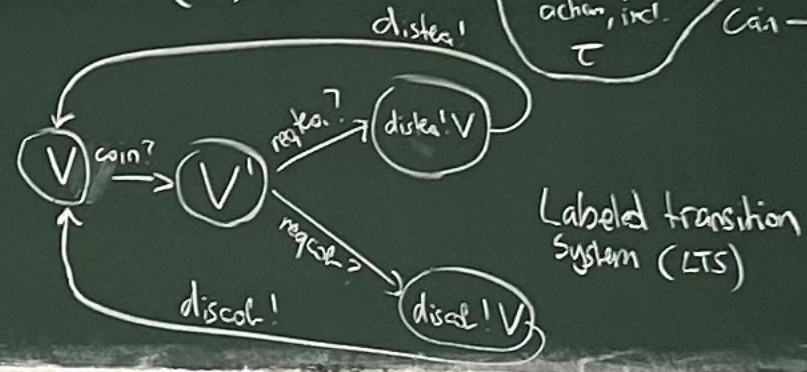
\includegraphics[width=0.7\linewidth]{images/1.png}
	% 	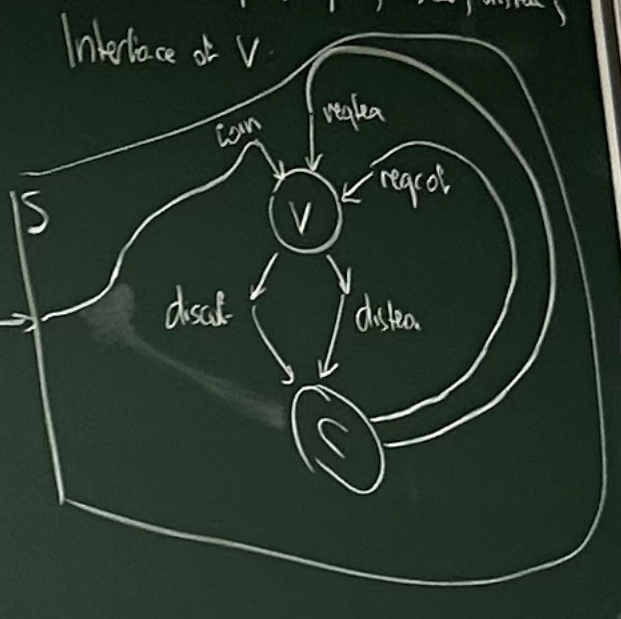
\includegraphics[width=0.7\linewidth]{images/2.png}
	% 	\caption{Interface of V}
	% \end{figure}
\end{example}





\begin{remark}
     CCS networks are Turing-complete but finite CCS networks are still infinite state but not Turing-complete.
\end{remark}

\begin{example}[Counter]
    Let $A \coloneq \{\inc, \dec, \zero\}$, then we define 
    \begin{align*}
        \Counter\coloneqq \left\{
            \begin{array}{l}
                C_0 = \inc?C_1 + \zero? C_0, \\
                C_1 = \inc?C_2 + \dec? C_0, \\
               C_2 = \inc?C_3 + \dec? C_1, \\
               \vdots
            \end{array}
        \right\}
    \end{align*}  
    and 
    \begin{align*}
        \semicounter \coloneq \{SC = \inc?(SC\parallel \dec?0)\}
    \end{align*}
   \begin{center}
 \begin{tikzpicture}[->, >=Stealth, node distance=2cm, thick, main/.style = {draw, ellipse}]
    % Nodes
  
    \node[main] (1) at (0, 0) {\small$SC$};
    \node[main] (2) at (3, 0) {\small$SC\parallel\dec?$};
    \node[main] (3) at (7, 0) {\small$(SC\parallel\dec?)\parallel\dec?$};
    \node (4) at (11, 0) {\small$\hdots$};

    % Edges
    \draw[bend left]  (1) to node[midway, above] {\small$\inc?$} (2) ;
    \draw[bend left]  (2) to node[midway, below] {\small$\dec?$} (1) ;
    \draw[bend left]  (2) to node[midway, above] {\small$\inc?$} (3) ;
    \draw[bend left]  (3) to node[midway, below] {\small$\dec?$} (2) ;
    \draw [bend left] (3) to node[midway, above] {\small$\inc?$} (4) ;
    \draw[bend left]  (4) to node[midway, below] {\small$\dec?$} (3) ;
   


\end{tikzpicture}
 \end{center}
\end{example}


\begin{definition}[Regular CCS Network]
    Regular (finite) CCS networks are defined by the following grammar. 
    Regular networks are finite state.
    \begin{align*}
        R &\Coloneqq O \;\mid\;  aP \;\mid\; R + R \\
        P &\Coloneqq R \;\mid\; C \\
        Q &\Coloneqq  P \;\mid\; Q \parallel  Q \;\mid\; (\nu a) Q
    \end{align*}
\end{definition}

\begin{remark}
    Regular CCS networks represent a finite set of CCS processes, each parallel composition of (possibly nested) sequential processes.
\end{remark}




\begin{theorem}[Laws]
For an appropriately chosen notion of equivalence, the following equation hold
\begin{align*}
    P + Q  &\approx Q + P, \; \\
    (P + Q) + R &\approx P + (Q + R), \;\\
    P + P &\approx P, \; \\
    P + O &\approx P
\end{align*}
In addition we have the \emph{expansion law}
\begin{align*}
    a \parallel  b \approx ab + ba
\end{align*}
\end{theorem}



\section{Labeled Transition Systems}

\begin{definition}[Labeled Transition Systems]
    A labeled transition systems (LTS) for a set of actions $A$ is a tuple $T\coloneqq (S, \to, )$ where $S$ is a set of states, and $\to \subseteq S\times A \times S$ is a labeled transition relation. It defines a finite or infinite directed graph whose edges are labeled by actions (including $\tau$ which is an invisible action).
\end{definition}


\begin{example}
    A process network $\mathcal{P}$ can be encoded as a LTS $T_{\mathcal{P}}$.
    We define $S$ to be the set of sub-processions that occur in  $\mathcal{P}$ closed under $\to$ and 
    $\to$ is given by the SOS rules. 
\end{example}


\begin{remark}
    A LTS $T=(S, \to)$ is finitely branching (for guarded process terms) if $A$ is finite and finite state if $S$ is finite. 
\end{remark}





\begin{exercise}
	Design a coffee machine that needs refilling after every second drink, together with a coffee preferring customer, and a second tea preferring customer that never refills. Give CCS network and the corresponding LTS (for all sub-processions).
\end{exercise}





% \begin{tikzpicture}[->, >=Stealth, node distance=2cm, thick, main/.style = {draw, circle}]
%     % Nodes
%     \node[main] (1) {A};
%     \node[main] (2) [below right of=1] {B};
%     \node[main] (3) [below left of=2] {C};
%     \node[main] (4) [below right of=2] {D};

%     % Edges
%     \draw[bend left] (1) to node[midway, above left] {2} (2);
%     \draw[bend left] (1) to node[midway, above right] {3} (3);
%     \draw[bend left] (2) to node[midway, below left] {1} (3);
%     \draw[bend left] (2) to node[midway, above right] {4} (4);
%     \draw[bend left] (3) to node[midway, below right] {5} (4);
% \end{tikzpicture}



% \paragraph{semanitcs}:
% $$\frac{}{aP \xrightarrow{a} P}$$
% $$\frac{P \xrightarrow{a} P'}{P + Q \xrightarrow{a} P' + Q, Q + P \xrightarrow{a} Q + P', P\parallel Q \xrightarrow{a} P'\parallel Q, Q\parallel P \xrightarrow{a} Q\parallel P'}$$
% $$\frac{P \xrightarrow{a?} P', Q \xrightarrow{a!} Q'}{P\parallel Q \xrightarrow{\tau} P' \parallel  Q', Q \parallel  P \xrightarrow{\tau} Q' \parallel  P'}$$ where $\tau$ is a fixed operator symbol
% $$\frac{P \xrightarrow{\mu} P'}{(\nu a)P \xrightarrow{\mu}(\nu a)P'}\mu \neq a!, a?$$ where $\mu$ is a meta variable standing for any action, including $\tau$

% \begin{example}
% 	continuation ...
	
% 	In figure \ref{lec18:pic2}.
% 	\begin{figure}[h]
% 		\label{lec18:pic2}
% 		\centering
% 		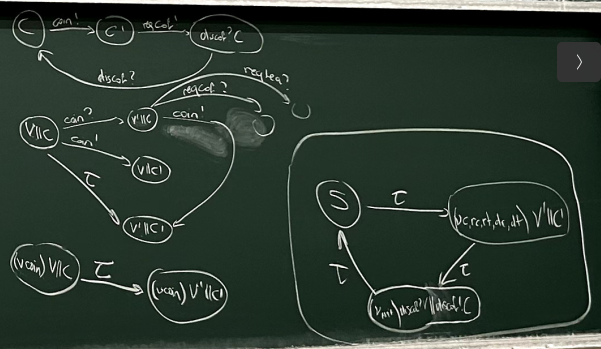
\includegraphics[width=0.7\linewidth]{images/3.png}
% 		\caption{Semantic of V}
% 	\end{figure}
% \end{example}



% \begin{example}
	
	
% 	counter =
% 	$\{C_0 = inc?C_1 + zero? C_0, C_1 = inc?C_2 + dec? C_0, C_2 = inc? C_3 + dec? C_1, ...\}$
	
% 	semi-counter:
% 	$\{SC = inc? (SC \parallel  dec?O)\}$
	
% 	See figure \ref{lec18:pic3}.
% 	\begin{figure}[h]
% 		\label{lec18:pic3}
% 		\centering
% 		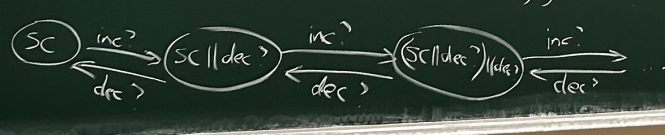
\includegraphics[width=0.7\linewidth]{images/4.png}
% 		\caption{Counter model}
% 	\end{figure}
% \end{example}



% Note:

% \paragraph{Regular finite CCS networks}
% $$R:= O | aP |R + R$$
% $$P := R | C$$
% $$Q :=  | Q \parallel  Q | (\nu a) Q$$

% finite set of CCS processes, each a parallel comb of seq processes.
% The regular networks are finite state.

% \begin{exercise}
% 	design a coffee machine that needs refilling after every second drink, together with a coffee preferring customer, and a second tea preferring customer that never refills. Give CCS network  + corresponding LTS (for all subprocessions)
% \end{exercise}



% \paragraph{"Laws" (equations)}
% $$ P + Q  \approx Q + P$$
% $$(P + Q) + R \approx P + (Q + R)$$
% $$P + P \approx P$$
% $$P + O \approx P$$

% Expansion law (simple form): $a \parallel  b \approx ab + ba$

% \subsection{LTS}
% LTS (for set $A$ of actions) $T = (S\text{(states)}, \rightarrow (subset S\times A \times S),)$
% finite or infinite directed graph whose edges are labeled by actions (including $\tau$(invisible action))

% Process network P $\rightarrow$ LTS $T_P$: 
% i) S = set of subprocessions that occur in P closed under $\rightarrow$, and ii) $\rightarrow$ = defined by SOS rules


% \paragraph{4 equivalence relations on LTS}
% \begin{itemize}
% 	\item $\eqiso$: isomorphism between LTS
% 	\item $\eqbis$: bisimilarity
% 	\item $\eqsim$: similarity
% 	\item $\eqlin$: language equivalance
% \end{itemize}

% Note: upper ones can result lower, but not the other way around.



